\section{Itération n°4}

\subsection{Objectif de l'itération}

Dans le cadre de cette itération 4, il nous est demandé d'implémenter un bruit "réel" causé par des trajets multiples. Cela nous permettra de nous rapprocher de la réalité et nous demandera de réfléchir à de nouvelles façons de décoder le message. Nous allons devoir modifier notre code afin que ce dernier puisse générer ce nouveau type de bruit dans le canal de transmission et gérer les problèmes au niveau du bruit et de sa puissance. Nous implémenterons donc une nouvelle classe que l'on appellera $TransmissionBruiteMultiTrajets$. Les bruits réels représentent l'association de trajets multiples, dispersion chromatique et de la chaleur (bruit thermique). 
Ci-dessous le schéma correspondant à l'itération n°4 (identique à la n°3) :

\begin{figure}[H]
\centering
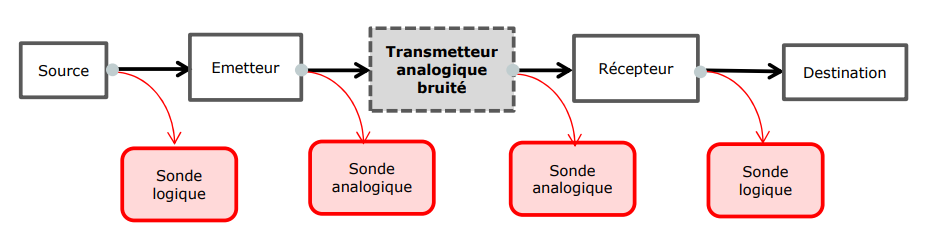
\includegraphics[width=1\textwidth]{image 21.png}
\caption{\label{fig:image21}Schéma de l'itération n°4.}
\end{figure}

Ci-dessous le schéma correspondant à l'ajout du bruit "réel" pour cette itération.

\begin{figure}[H]
\centering
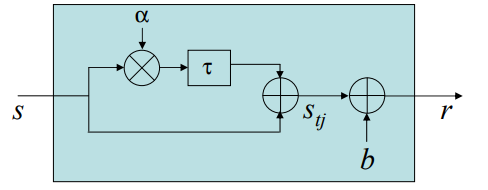
\includegraphics[width=1\textwidth]{image 22.png}
\caption{\label{fig:image22}Schéma d'ajout de bruit de l'itération n°4.}
\end{figure}

\subsubsection{correction des itérations précédentes}

Nous avons optimisé notre code précédent, cela nous permet de gagner du temps de calcul lorsque nous simulons un nombre important d'échantillons.  

\subsection{Organisation}

 Nous allons devoir créer de nouveaux éléments par rapport au code de l'itération précédente. Ces modifications devrons nous aider à lancer le programme tout en prenant en compte la génération de ce nouveau type de bruit que nous retrouvons dans les canaux de transmission suite aux différentes perturbations. Nous ne devrions pas avoir d'erreurs sur notre code cependant, nous devrions pouvoir observer les conséquences de l'ajout du bruit "réel" sur le signal. Nous pourrions voir tout cela grâce à la simulation des signaux mais également à de graphes. Pour vérifier le bon fonctionnement de notre code nous nous appuierons donc sur ces dernières. Dans le but d'effectuer ces modifications, nous avons amélioré le diagramme de Gant que nous avions utilisé lors de nos précédentes itérations. Voici à quoi il ressemble pour cette itération.
 
\subsection{Procédure de développement}

Développer un code lisible est indispensable pour avoir un programme efficace et facile à maintenir. Nous avons donc décidé de faire hériter notre classe $TransmetteurBruiteMultiTrajets$ par $TransmetteurBruiteAnalogique$. Cela nous permet d'ajouter du bruit à notre signal avec multi-trajet facilement sans avoir à connecter un transmetteur bruité avec un transmetteur multi-trajet. On évite alors quelques copies et nous gagnons alors en performances. Le plus important est de fragmenter le code de sorte à avoir une méthode par fonctionnalité. Cela nous permet de mieux nous organiser et de mieux travailler en collaboration sur le même code. A ce stade du projet, l'utilisation de git nous à permis également de diviser les taches en travaillant sur une branche par fonctionnalité. Nous pouvons donc chacun de notre coté altérer le code sans causer de problème aux autres.

\begin{figure}[H]
\centering
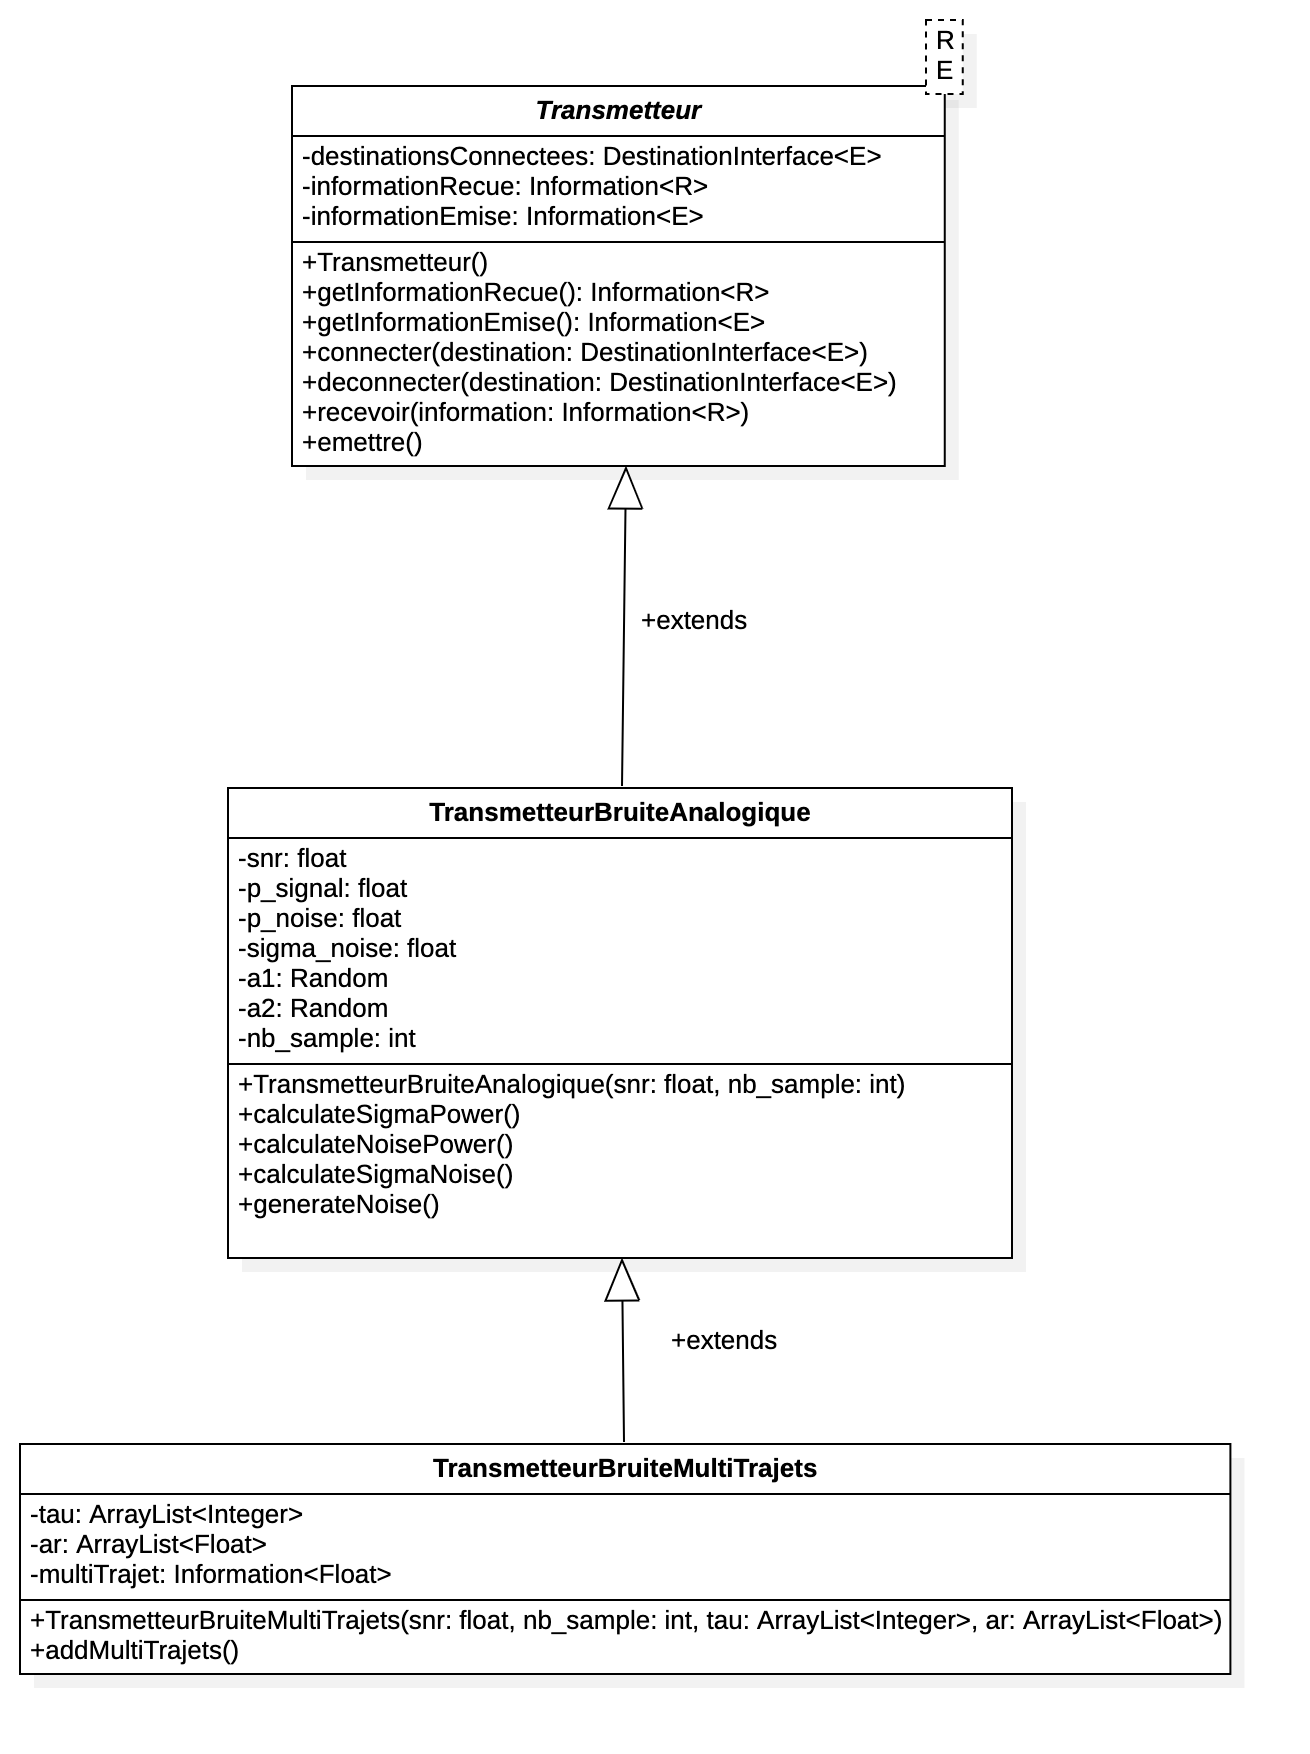
\includegraphics[width=\textwidth]{img/transm_multiTrajets.png}
\caption{\label{fig:image23}Diagramme de classes de l'implémentation du multi-trajet.}
\end{figure}

\pagebreak

\subsection{Trajets multiples}

L'objectif de cette itération est de voir l'impact de trois facteurs différents sur le récepteur. 

\subsubsection{impact des trajets multiples}

Nous allons nous intéresser maintenant à l'impact des trajets multiples. Pour ce faire nous allons effectuer deux simulations où le retard sera de 0 et les trajets auront la même amplitude. Le message émis est le même.

\begin{figure}[H]
\centering
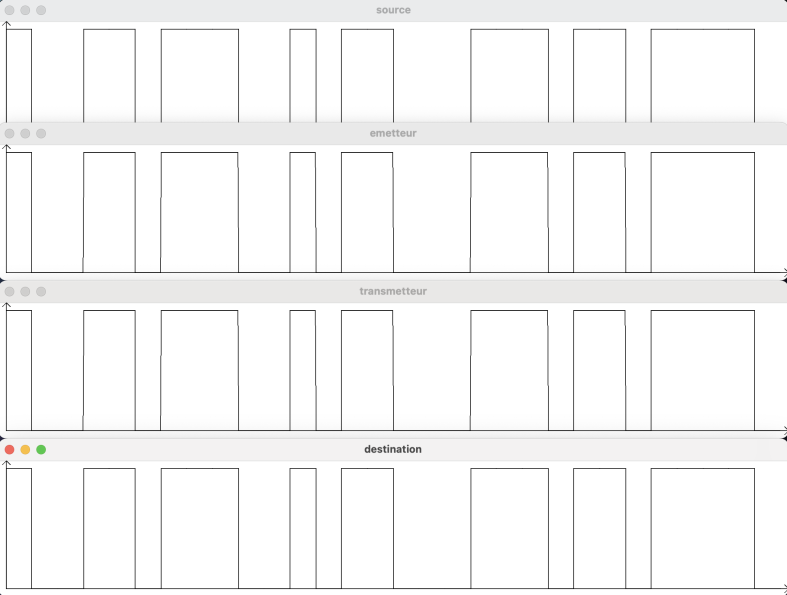
\includegraphics[width=\textwidth]{img/nulledecalage.png}
\caption{\label{fig:image25}Simulation avec 2 trajets multiples avec amplitude à 0}
\end{figure}

\begin{figure}[H]
\centering
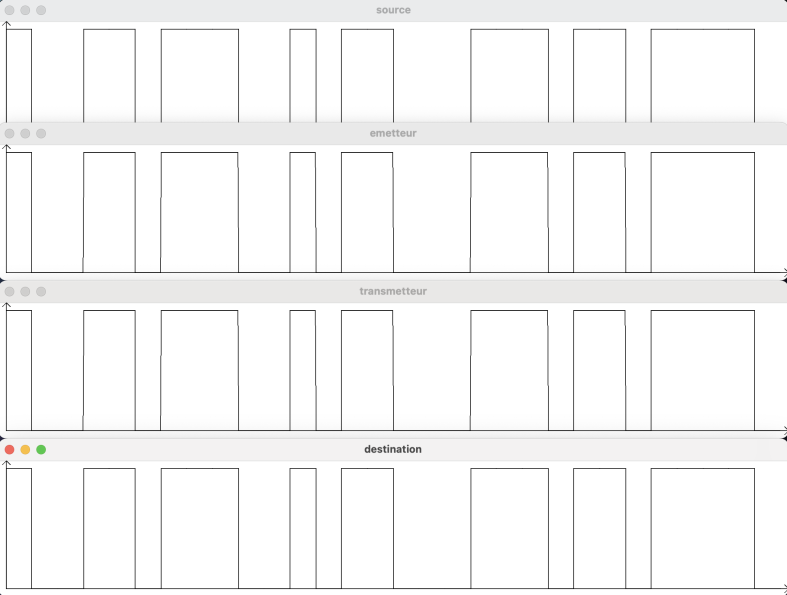
\includegraphics[width=\textwidth]{img/nulledecalage.png}
\caption{\label{fig:image25}Simulation avec 5 trajets multiples avec amplitude à 0}
\end{figure}

On constate que le TEB est de 0 dans les deux cas. Le multi trajet n'a pas d'impact s'il n'y a pas de retard ou de changement d'amplitude.


\subsubsection{impact du retard et de l'atténuation}
Dans cette partie, nous allons étudier l'impact du retard et de l'atténuation lors de trajets multiples. Nos signaux vont être reçu par le récepteur avec un décalage plus ou moins important. Tout d'abord voici la simulation avec deux trajets (le trajet direct et 1 trajet retardé) ayant la même amplitude et un retard de 20 échantillons.

(-s  -seed  99  -mess  30  -form  NRZ  -nbEch  100  -ampl  0  2  -snrpb  1000  -ti  20 0.9)

\begin{figure}[H]
\centering
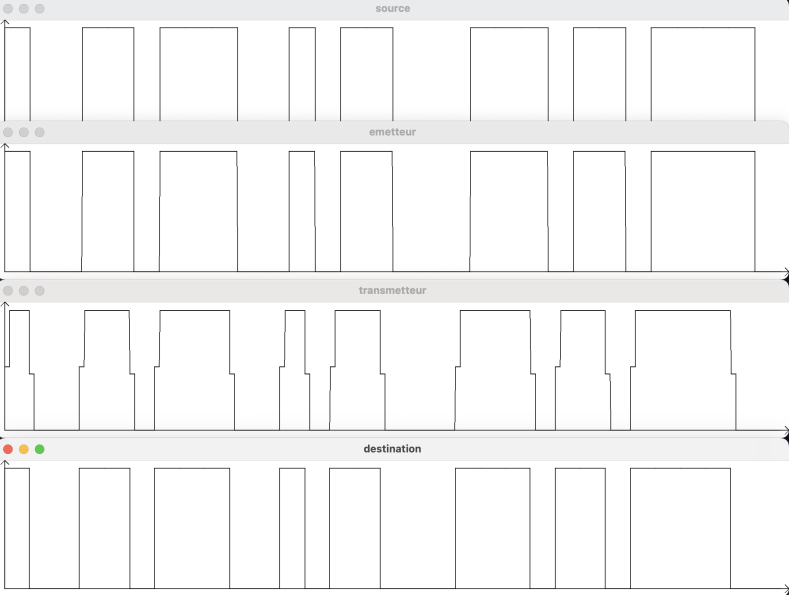
\includegraphics[width=\textwidth]{img/peuretard.png}
\caption{\label{fig:image25}Simulation avec 2 trajets multiples et un léger retard}
\end{figure}

On observe que le signal en sortie d'émetteur et de récepteur est le même. Le peu de retard n'impacte pas nos le décodage en réception. On effectue une nouvelle simulation mais cette fois ci, le deuxième signal aura un décalage de 80 échantillons.

(-s  -seed  99  -mess  30  -form  NRZ  -nbEch  100  -ampl  0  2  -snrpb  1000  -ti  80 0.9)

\begin{figure}[H]
\centering
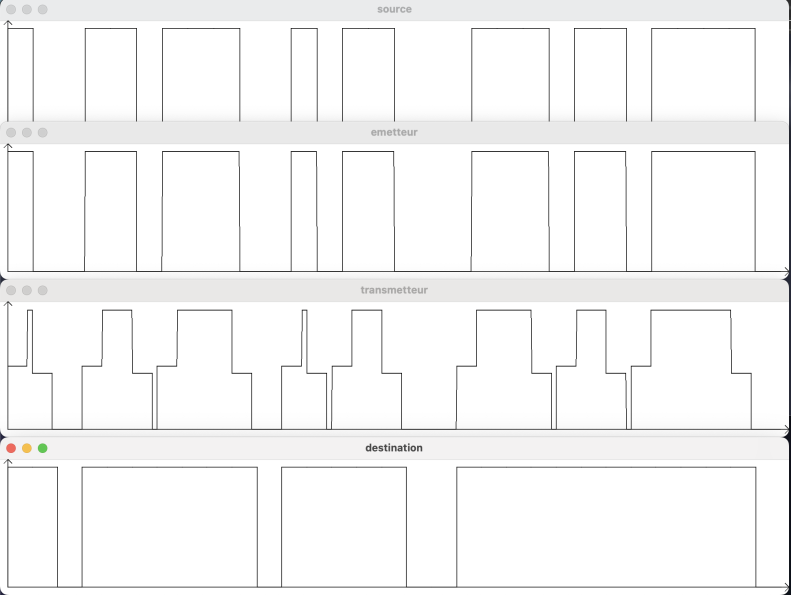
\includegraphics[width=\textwidth]{img/beaudecalage.png}
\caption{\label{fig:image25}Simulation avec 2 trajets multiples et un retard d'un demi symbole}
\end{figure}

Cette fois-ci, on n'obtient plus le même signal qu'à l'origine. Cela conclut le fait que le retard est un facteur important à prendre en compte lors de transmission multi-trajets. Une mauvaise gestion de ce dernier peut rendre notre système de transmission inopérant. 
Pour finir, nous allons étudier l'impact des amplitudes des multi-trajets. Pour ce faire, nous allons reprendre le multi-trajet précédents (même retard) mais nous allons baisser l'amplitude des signaux retardés de  80\%. 

( -s  -seed  99  -mess  30  -form  NRZ  -nbEch  100  -ampl  0  2  -snrpb  1000  -ti  100  0.1  100  0.1)

\begin{figure}[H]
\centering
\includegraphics[width=\textwidth]{img/atténuation.png}
\caption{\label{fig:image25}Simulation avec 2 trajets multiples retardé avec une amplitude plus importante pour le signal non décalé}
\end{figure}

On remarque que les signaux retardés n'interfèrent plus avec notre signal initial. Notre décodeur retrouve le même signal qu'à l'émission. Ainsi, si les signaux décalés ont une amplitude beaucoup plus faible que le signal non retardé, il n'y aura pas d'impact à la réception.
\subsubsection{Performances du code}

Dans une optique de performances plus rapides, nous avons réalisé un changement majeur dans le code de la classe $Information$. Cette modification consiste au passage des $LinkedList$ vers des $ArrayList$. Cette mise à jour du code est significative particulièrement a cause de notre façon de traiter les informations. Nous écrivons beaucoup dans de nouvelles listes sans particulièrement les modifier. Les LinkedList étant performantes pour la modification de données dans le tableau, cela ne nous est pas utile dans notre cas d'usage. Les ArrayList quant à elles sont très performantes mais beaucoup plus lentes pour la modification d'informations à l'intérieur de la liste. Ces opérations n'étant rarement voir jamais réalisés il alors logique pour notre groupe de changer de type de liste. La classe $Information$ nous facilite la vie car, en effet cela ne nous demande que quelques lignes à modifier dans le programme.

\subsection{Conclusion}

Pour conclure cette itération, nous avons pu étudier sur les multi-trajets. Grâce aux simulations, nous avons pu comprendre l'impact du retard et des atténuations sur le récepteur. Cela nous a permis de comprendre l'importance de ces paramètres et la nécessité d'avoir des correcteurs à ceux-ci.
Dans l'itération suivante, nous allons implémenter un codage de canal afin de corriger les  éventuels erreurs à la réception. 